\documentclass[tikz, border=2mm]{standalone}
\usepackage{amsmath}
\usetikzlibrary{automata, positioning, arrows}
\tikzset{
  ->, % makes the edges directed
  >=stealth', % makes the arrow heads bold
  node distance=3cm, % specifies the minimum distance between two nodes. Change if necessary.
  every state/.style={thick}, % sets the properties for each ’state’ node
  initial text=, % sets the text that appears on the start arrow
}

\begin{document}

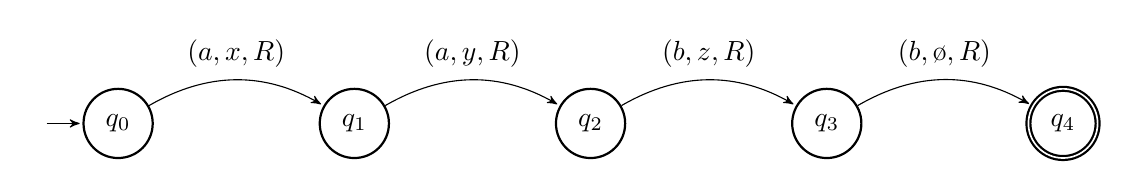
\begin{tikzpicture}[shorten >=1pt, on grid, auto]
  \node[state, initial] (0) {$q_0$};
  \node[state, right of=0] (1) {$q_1$};
  \node[state, right of=1] (2) {$q_2$};
  \node[state, right of=2] (3) {$q_3$};
  \node[state, right of=3, accepting] (4) {$q_4$};
  
  \draw  
    (0) edge[bend left, above] node[above]{$
    \begin{aligned}
      (a, x, R)
    \end{aligned}$} (1);
   
  \draw  
    (1) edge[bend left, above] node[above]{$
    \begin{aligned}
      (a, y, R)
    \end{aligned}$} (2);
    
  \draw  
    (2) edge[bend left, above] node[above]{$
    \begin{aligned}
      (b, z, R)
    \end{aligned}$} (3);   

  \draw  
    (3) edge[bend left, above] node[above]{$
    \begin{aligned}
      (b, \o{}, R)
    \end{aligned}$} (4);   

 
\end{tikzpicture}

\end{document}